\section{Referencia de la Clase Inventarios\-Sub\-Form}
\label{classInventariosSubForm}\index{InventariosSubForm@{InventariosSubForm}}
Muestra y administra las l\'{\i}neas de detalle del listado de inventarios.  


{\tt \#include $<$inventariosview.h$>$}

Diagrama de herencias de Inventarios\-Sub\-Form\begin{figure}[H]
\begin{center}
\leavevmode
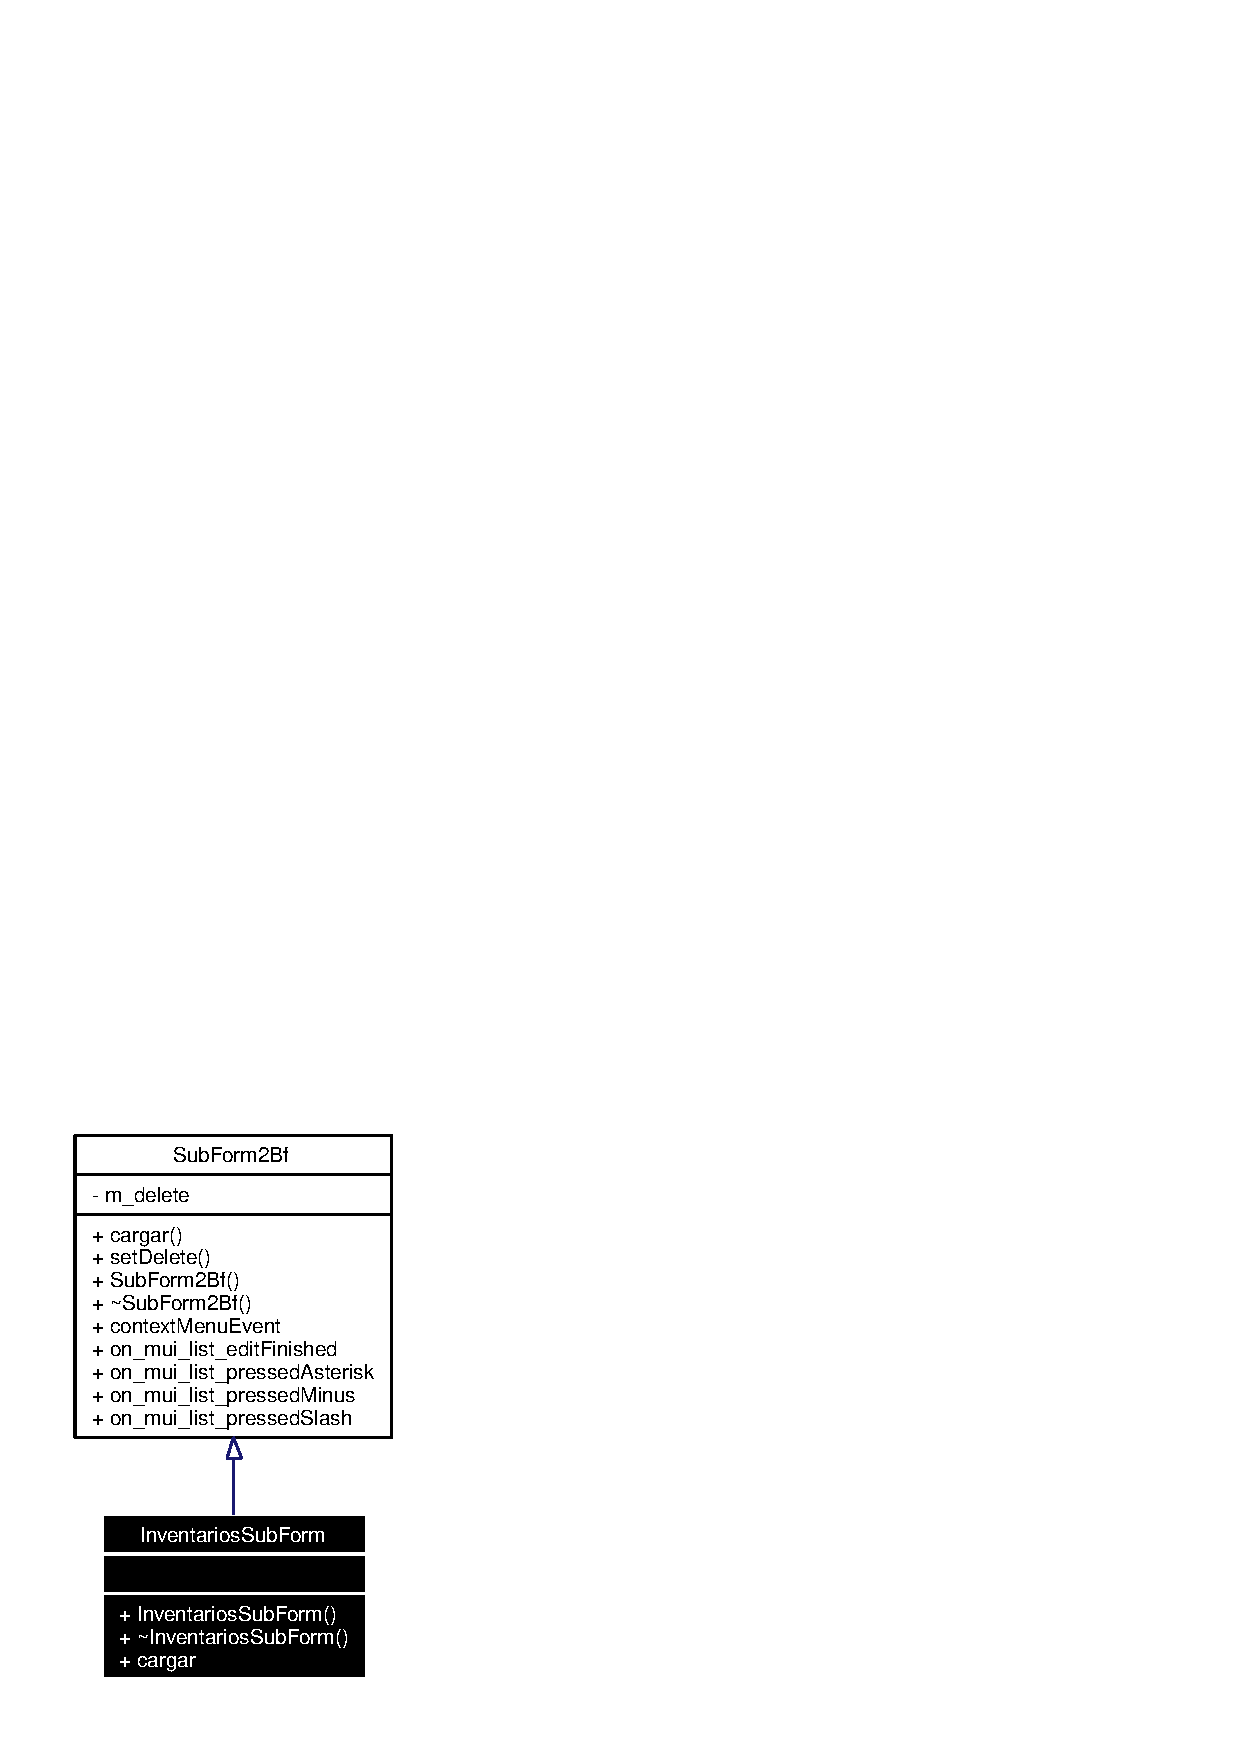
\includegraphics[width=94pt]{classInventariosSubForm__inherit__graph}
\end{center}
\end{figure}
Diagrama de colaboraci\'{o}n para Inventarios\-Sub\-Form:\begin{figure}[H]
\begin{center}
\leavevmode
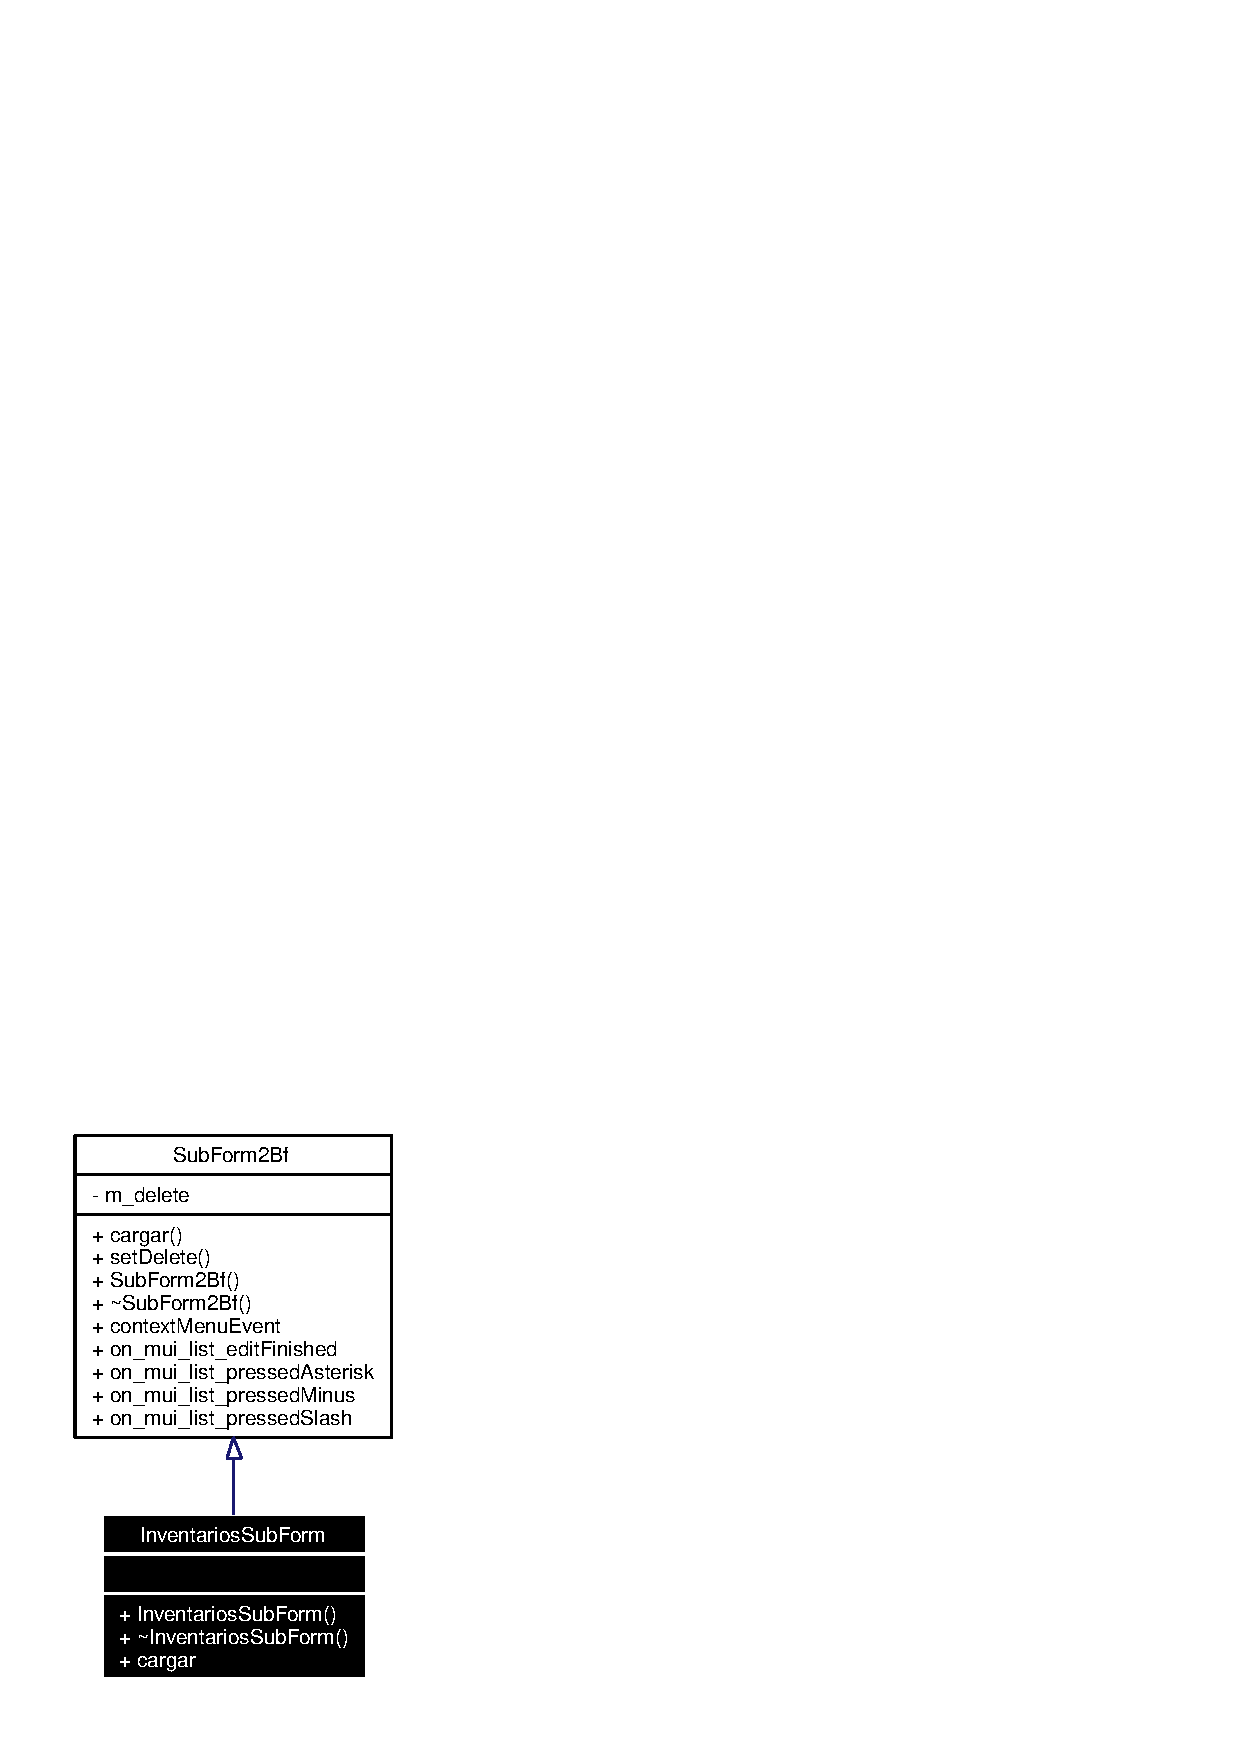
\includegraphics[width=94pt]{classInventariosSubForm__coll__graph}
\end{center}
\end{figure}
\subsection*{Slots p\'{u}blicos}
\begin{CompactItemize}
\item 
virtual void {\bf cargar} ()\label{classInventariosSubForm_i0}

\end{CompactItemize}
\subsection*{M\'{e}todos p\'{u}blicos}
\begin{CompactItemize}
\item 
{\bf Inventarios\-Sub\-Form} (QWidget $\ast$parent=0)
\end{CompactItemize}


\subsection{Descripci\'{o}n detallada}
Muestra y administra las l\'{\i}neas de detalle del listado de inventarios. 



\subsection{Documentaci\'{o}n del constructor y destructor}
\index{InventariosSubForm@{Inventarios\-Sub\-Form}!InventariosSubForm@{InventariosSubForm}}
\index{InventariosSubForm@{InventariosSubForm}!InventariosSubForm@{Inventarios\-Sub\-Form}}
\subsubsection{\setlength{\rightskip}{0pt plus 5cm}Inventarios\-Sub\-Form::Inventarios\-Sub\-Form (QWidget $\ast$ {\em parent} = {\tt 0})}\label{classInventariosSubForm_a0}


============================================================================= SUBFORMULARIO ============================================================================= 

La documentaci\'{o}n para esta clase fu\'{e} generada a partir de los siguientes archivos:\begin{CompactItemize}
\item 
inventariosview.h\item 
inventariosview.cpp\end{CompactItemize}
